% Created by tikzDevice version 0.6.2-92-0ad2792 on 2013-02-06 15:47:33
% !TEX encoding = UTF-8 Unicode
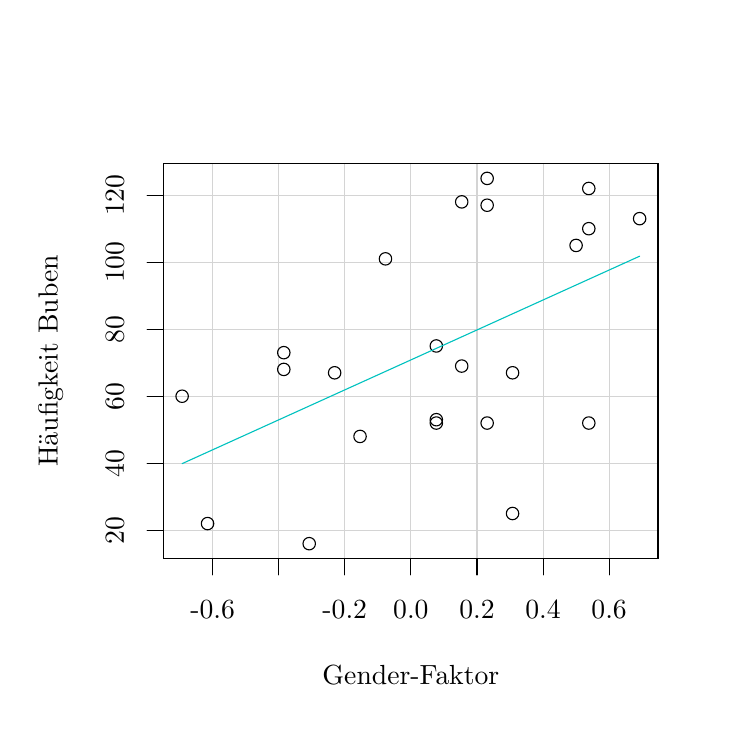
\begin{tikzpicture}[x=1pt,y=1pt]
\definecolor[named]{fillColor}{rgb}{1.00,1.00,1.00}
\path[use as bounding box,fill=fillColor,fill opacity=0.00] (0,0) rectangle (252.94,252.94);
\begin{scope}
\path[clip] (  0.00,  0.00) rectangle (252.94,252.94);
\definecolor[named]{drawColor}{rgb}{0.00,0.00,0.00}

\path[draw=drawColor,line width= 0.4pt,line join=round,line cap=round] ( 66.83, 61.20) -- (210.11, 61.20);

\path[draw=drawColor,line width= 0.4pt,line join=round,line cap=round] ( 66.83, 61.20) -- ( 66.83, 55.20);

\path[draw=drawColor,line width= 0.4pt,line join=round,line cap=round] ( 90.71, 61.20) -- ( 90.71, 55.20);

\path[draw=drawColor,line width= 0.4pt,line join=round,line cap=round] (114.59, 61.20) -- (114.59, 55.20);

\path[draw=drawColor,line width= 0.4pt,line join=round,line cap=round] (138.47, 61.20) -- (138.47, 55.20);

\path[draw=drawColor,line width= 0.4pt,line join=round,line cap=round] (162.35, 61.20) -- (162.35, 55.20);

\path[draw=drawColor,line width= 0.4pt,line join=round,line cap=round] (186.23, 61.20) -- (186.23, 55.20);

\path[draw=drawColor,line width= 0.4pt,line join=round,line cap=round] (210.11, 61.20) -- (210.11, 55.20);

\node[text=drawColor,anchor=base,inner sep=0pt, outer sep=0pt, scale=  1.00] at ( 66.83, 39.60) {-0.6};

\node[text=drawColor,anchor=base,inner sep=0pt, outer sep=0pt, scale=  1.00] at (114.59, 39.60) {-0.2};

\node[text=drawColor,anchor=base,inner sep=0pt, outer sep=0pt, scale=  1.00] at (138.47, 39.60) {0.0};

\node[text=drawColor,anchor=base,inner sep=0pt, outer sep=0pt, scale=  1.00] at (162.35, 39.60) {0.2};

\node[text=drawColor,anchor=base,inner sep=0pt, outer sep=0pt, scale=  1.00] at (186.23, 39.60) {0.4};

\node[text=drawColor,anchor=base,inner sep=0pt, outer sep=0pt, scale=  1.00] at (210.11, 39.60) {0.6};

\path[draw=drawColor,line width= 0.4pt,line join=round,line cap=round] ( 49.20, 71.32) -- ( 49.20,192.41);

\path[draw=drawColor,line width= 0.4pt,line join=round,line cap=round] ( 49.20, 71.32) -- ( 43.20, 71.32);

\path[draw=drawColor,line width= 0.4pt,line join=round,line cap=round] ( 49.20, 95.54) -- ( 43.20, 95.54);

\path[draw=drawColor,line width= 0.4pt,line join=round,line cap=round] ( 49.20,119.76) -- ( 43.20,119.76);

\path[draw=drawColor,line width= 0.4pt,line join=round,line cap=round] ( 49.20,143.98) -- ( 43.20,143.98);

\path[draw=drawColor,line width= 0.4pt,line join=round,line cap=round] ( 49.20,168.19) -- ( 43.20,168.19);

\path[draw=drawColor,line width= 0.4pt,line join=round,line cap=round] ( 49.20,192.41) -- ( 43.20,192.41);

\node[text=drawColor,rotate= 90.00,anchor=base,inner sep=0pt, outer sep=0pt, scale=  1.00] at ( 34.80, 71.32) {20};

\node[text=drawColor,rotate= 90.00,anchor=base,inner sep=0pt, outer sep=0pt, scale=  1.00] at ( 34.80, 95.54) {40};

\node[text=drawColor,rotate= 90.00,anchor=base,inner sep=0pt, outer sep=0pt, scale=  1.00] at ( 34.80,119.76) {60};

\node[text=drawColor,rotate= 90.00,anchor=base,inner sep=0pt, outer sep=0pt, scale=  1.00] at ( 34.80,143.98) {80};

\node[text=drawColor,rotate= 90.00,anchor=base,inner sep=0pt, outer sep=0pt, scale=  1.00] at ( 34.80,168.19) {100};

\node[text=drawColor,rotate= 90.00,anchor=base,inner sep=0pt, outer sep=0pt, scale=  1.00] at ( 34.80,192.41) {120};

\path[draw=drawColor,line width= 0.4pt,line join=round,line cap=round] ( 49.20, 61.20) --
	(227.75, 61.20) --
	(227.75,203.75) --
	( 49.20,203.75) --
	( 49.20, 61.20);
\end{scope}
\begin{scope}
\path[clip] (  0.00,  0.00) rectangle (252.94,252.94);
\definecolor[named]{drawColor}{rgb}{0.00,0.00,0.00}

\node[text=drawColor,anchor=base,inner sep=0pt, outer sep=0pt, scale=  1.00] at (138.47, 15.60) {Gender-Faktor};

\node[text=drawColor,rotate= 90.00,anchor=base,inner sep=0pt, outer sep=0pt, scale=  1.00] at ( 10.80,132.47) {Häufigkeit Buben};
\end{scope}
\begin{scope}
\path[clip] ( 49.20, 61.20) rectangle (227.75,203.75);
\definecolor[named]{drawColor}{rgb}{0.83,0.83,0.83}

\path[draw=drawColor,line width= 0.4pt,line join=round,line cap=round] ( 66.83, 61.20) -- ( 66.83,203.75);

\path[draw=drawColor,line width= 0.4pt,line join=round,line cap=round] ( 90.71, 61.20) -- ( 90.71,203.75);

\path[draw=drawColor,line width= 0.4pt,line join=round,line cap=round] (114.59, 61.20) -- (114.59,203.75);

\path[draw=drawColor,line width= 0.4pt,line join=round,line cap=round] (138.47, 61.20) -- (138.47,203.75);

\path[draw=drawColor,line width= 0.4pt,line join=round,line cap=round] (162.35, 61.20) -- (162.35,203.75);

\path[draw=drawColor,line width= 0.4pt,line join=round,line cap=round] (186.23, 61.20) -- (186.23,203.75);

\path[draw=drawColor,line width= 0.4pt,line join=round,line cap=round] (210.11, 61.20) -- (210.11,203.75);

\path[draw=drawColor,line width= 0.4pt,line join=round,line cap=round] ( 49.20, 71.32) -- (227.75, 71.32);

\path[draw=drawColor,line width= 0.4pt,line join=round,line cap=round] ( 49.20, 95.54) -- (227.75, 95.54);

\path[draw=drawColor,line width= 0.4pt,line join=round,line cap=round] ( 49.20,119.76) -- (227.75,119.76);

\path[draw=drawColor,line width= 0.4pt,line join=round,line cap=round] ( 49.20,143.98) -- (227.75,143.98);

\path[draw=drawColor,line width= 0.4pt,line join=round,line cap=round] ( 49.20,168.19) -- (227.75,168.19);

\path[draw=drawColor,line width= 0.4pt,line join=round,line cap=round] ( 49.20,192.41) -- (227.75,192.41);
\end{scope}
\begin{scope}
\path[clip] (  0.00,  0.00) rectangle (252.94,252.94);
\definecolor[named]{drawColor}{rgb}{0.00,0.00,0.00}

\path[draw=drawColor,line width= 0.4pt,line join=round,line cap=round] ( 49.20, 61.20) --
	(227.75, 61.20) --
	(227.75,203.75) --
	( 49.20,203.75) --
	( 49.20, 61.20);
\end{scope}
\begin{scope}
\path[clip] ( 49.20, 61.20) rectangle (227.75,203.75);
\definecolor[named]{drawColor}{rgb}{0.00,0.00,0.00}

\path[draw=drawColor,line width= 0.4pt,line join=round,line cap=round] (202.76,180.30) circle (  2.25);

\path[draw=drawColor,line width= 0.4pt,line join=round,line cap=round] (156.84,130.66) circle (  2.25);

\path[draw=drawColor,line width= 0.4pt,line join=round,line cap=round] (175.21,128.23) circle (  2.25);

\path[draw=drawColor,line width= 0.4pt,line join=round,line cap=round] (166.03,188.78) circle (  2.25);

\path[draw=drawColor,line width= 0.4pt,line join=round,line cap=round] (166.03,198.47) circle (  2.25);

\path[draw=drawColor,line width= 0.4pt,line join=round,line cap=round] (202.76,194.83) circle (  2.25);

\path[draw=drawColor,line width= 0.4pt,line join=round,line cap=round] (198.17,174.25) circle (  2.25);

\path[draw=drawColor,line width= 0.4pt,line join=round,line cap=round] (166.03,110.07) circle (  2.25);

\path[draw=drawColor,line width= 0.4pt,line join=round,line cap=round] (221.13,183.93) circle (  2.25);

\path[draw=drawColor,line width= 0.4pt,line join=round,line cap=round] (147.66,110.07) circle (  2.25);

\path[draw=drawColor,line width= 0.4pt,line join=round,line cap=round] (129.29,169.40) circle (  2.25);

\path[draw=drawColor,line width= 0.4pt,line join=round,line cap=round] (110.92,128.23) circle (  2.25);

\path[draw=drawColor,line width= 0.4pt,line join=round,line cap=round] (156.84,189.99) circle (  2.25);

\path[draw=drawColor,line width= 0.4pt,line join=round,line cap=round] (120.10,105.23) circle (  2.25);

\path[draw=drawColor,line width= 0.4pt,line join=round,line cap=round] ( 92.55,135.50) circle (  2.25);

\path[draw=drawColor,line width= 0.4pt,line join=round,line cap=round] ( 55.81,119.76) circle (  2.25);

\path[draw=drawColor,line width= 0.4pt,line join=round,line cap=round] ( 92.55,129.45) circle (  2.25);

\path[draw=drawColor,line width= 0.4pt,line join=round,line cap=round] (147.66,137.92) circle (  2.25);

\path[draw=drawColor,line width= 0.4pt,line join=round,line cap=round] (202.76,110.07) circle (  2.25);

\path[draw=drawColor,line width= 0.4pt,line join=round,line cap=round] (147.66,111.28) circle (  2.25);

\path[draw=drawColor,line width= 0.4pt,line join=round,line cap=round] (175.21, 77.38) circle (  2.25);

\path[draw=drawColor,line width= 0.4pt,line join=round,line cap=round] (101.73, 66.48) circle (  2.25);

\path[draw=drawColor,line width= 0.4pt,line join=round,line cap=round] ( 65.00, 73.74) circle (  2.25);
\definecolor[named]{drawColor}{rgb}{0.00,0.76,0.75}

\path[draw=drawColor,line width= 0.4pt,line join=round,line cap=round] ( 55.81, 95.40) --
	(221.13,170.36);
\end{scope}
\end{tikzpicture}
